\chapter{Interactive Musical Score}

\section{Introduction}

Learning to read music from the score is an essential part of Western classical music
training. Traditionally, children learn the different music notes by singing or playing
notes on an instrument, guided by a teacher. We envision a way for children to learn
the correspondence between notation and sound by directly touching the score.
The Interactive Score is effortless to use and allows children to make discoveries on
their own. The correspondence between the visual, the tactile, and the sound can aid
in learning.

In this work, we introduce the Interactive Score, a novel instrumental device for children's solfege
learning. Paper scores are overlaid onto a staff drawn with conductive ink and
connected to an Adafruit musical box. Pressing a note in the score triggers its sound,
and running fingers over the notes plays a melody.


\subsection*{Motivation}

\section{Related work}

\subsection{Context} 

A review of music theory pedagogy over the past decade reveals many criticisms of the way music theory courses have been taught. Other concerns include issues such as whether to take a harmonic, melodic, or compositional approach to teaching theory. The early involvement of students in creative thinking about harmony, melody, and rhythm determines in part its success in the theoretical program \cite{bland1977college}. The development of a feeling for the mastery of the preliminaries to music as well as the presentation of the basics are the prerequisites for a successful future theoretical education.

But out of the large number of students who embark on learning music, only a small portion retain the courage and motivation to continue their studies to the end.
For example, out of 100 French people aged 15 and over, a study recorded that only 30\% of the musicians who have learned music continue to practice their instrument during their their lives \cite{amateurs}. 

It is pointless and frustrating for students to be pushed too quickly into advanced and sophisticated theory without visualizing audibly what they are studying.

\subsection{Approaches}

Music theory courses can take many forms. There are many approaches to developing musicianship skills. Teachers often choose between traditional or more contemporary approaches.

\paragraph*{Traditional approach}

Traditional music lessons prepare students to read, write and perform music from the work of great academic composers. It produces excellent results in terms of sight-reading skills. But a significant number of students leave these music studies because of their lack of enjoyment of the method.


\paragraph*{Contemporary approach}
Contemporary music lessons are paired with instrumental lessons (usually piano or guitar). They do not require music reading or theory. These lessons focus on skill, musicality, and more intuitive learning methods. They require the student to have a good ear for music and a sense of rhythm. The contemporary approach is beneficial for students who have difficulty visualizing with theory classes. They are able to play real pieces only a few months after starting their lessons.  


The actual major advice if a student has any problem understanding music theory, is to study the theory on the piano. Intervals and harmonies are easier to understand on a piano first, as is all the rest of the theory.

\subsection{Musical Mental Projection}

Musical imagery, or the ability to create an image of sound in our minds, is an essential
skill for all musicians. For example, brass, winds, strings, and singers imagine the
pitch of an upcoming note to make it easier to play it and determine the distance from
the previous note
\cite{zatorre2005mental}. Composers and arrangers also use musical imagery when creating
a new piece. Musical imagery training has been shown to improve the ability to follow
the upward and downward movements of the tonal contour of a musical phrase or
imagined tune
\cite{weber1986musical}.

Ear training" (or solfege) has traditionally been part of the curriculum of most music
schools. An important part of solfege is the ability to read music notation and imagine
how it is supposed to sound. We are interested in teaching this skill to children.

\subsection{Tangible Interactive Medias for Music Practise}

Many projects aim at getting a child involved in the world of music. But few of them consist of a tangible interactive media for music discovery.

For example, Zigelbaum et al. investigated how electronic instruments can engage young learners in learning to make music. Their project was the development of different tools involving movement, linking it to a sound. They created a trampoline, an interactive matrix, or musical bracelets \cite{zigelbaum2006bodybeats}.

Xiao Xiao et Al. propose an understanding of the essential workings of music without going into the details of music theory \cite{xiao2014andante}.
The authors expose a new technique for visualizing musical motion on a piano keyboard. The technique, called Andante, uses walking figures that move along the keyboard to represent the movement of musical phrases. The results of their user test showed that the participants found the Andante animation to be significantly more informative and engaging than the video without animation.

\begin{marginfigure}
    \centering
    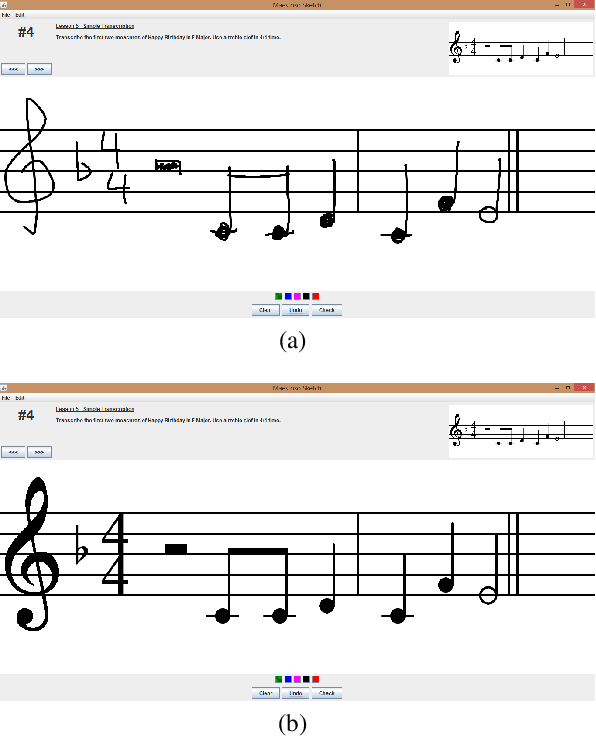
\includegraphics{images/maestoso.png}
    \caption{Maestoso Educational
    Sketching Tool for Learning Music Theory}
    \label{fig:taele2015maestoso}
\end{marginfigure}

The work of Taele et al. \cite{taele2015maestoso} \ref{fig:taele2015maestoso} describes the practical and cognitive benefits of learning music theory for both musicians and non-musicians. The paper proposes an intelligent educational tool designed to help students learn music theory. The tool, called Maestoso, utilizes sketch-based interaction and machine learning techniques to provide personalized feedback to the user.
The paper first introduces the importance of music education and the challenges students face when learning music theory, such as the abstract nature of music concepts and the difficulty of translating musical ideas into notation.
Maestoso is based on a sketching interface that allows users to draw musical notes, chords, and melodies using a stylus or finger. The program uses machine learning algorithms to recognize the user's sketches and provide feedback on their accuracy and completeness.

\begin{marginfigure}
    \centering
    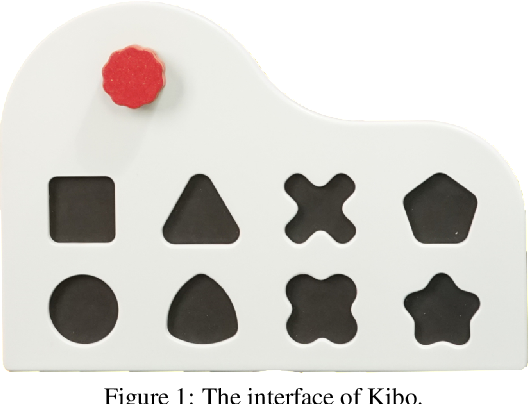
\includegraphics{images/IS_kibo.png}
    \caption{The interface of Kibo}
    \label{fig:amico2020kibo}
\end{marginfigure}

Amico et al. discuss the development of a new type of MIDI controller designed for music education \cite{amico2020kibo}. The device, called Kibo, is a tangible user interface that allows students to interact with music in a physical, intuitive way.
The authors introduce the concept of tangible user interfaces and explain how they can be used to create more immersive and interactive learning experiences.
The device includes a set of modular blocks that can be rearranged and customized to create different musical experiences.

Implementing such systems is often fully digital and interactive through a screen. Some projects aim to teach children music theory or interact with notes to compose, learn and experiment. Most of these projects are applications that users can download on smartphones or tablets. The relationship with the tangible paper score is gradually lost and could soon be entirely replaced by digital interaction.

One solution is to use conductive ink to keep a tool in paper form without losing its interactive aspect. Conductive inks, paints, and varnishes are liquids containing metal particles, conductive polymers, or graphite. They are specifically designed to conduct electricity.

Inkjet printing has been used to pattern organic semiconductors \cite{kim2008heterogeneous}, metal contacts on organic semiconductors \cite{khan2019soft} \cite{wessely2020sprayable}, and metallic structures that require minimal further processing. Researchers such as Ahn et al. used conductive ink printing to realize metallic connections between functional components of flexible devices. 

\begin{marginfigure}
    \centering
    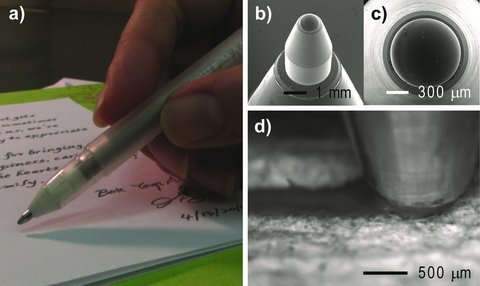
\includegraphics{images/IS_pen-on-paper.jpg}
    \caption{Pen-on-Paper Flexible Electronics. a) Optical image of a rollerball pen loaded with a conductive silver ink. b) and c) side and top views of the rollerball pen. d) Optical image of the rollerball pen tip writing a conductive silver track}
    \label{fig:IS_pen-on-paper}
\end{marginfigure}

Another project like that of Russo et al. \cite{IS_pen-on-paper} has resulted in an optical image of a flexible paper display containing a LED array. It takes the form of a multi-color 25 × 16 LED array connected to the printed silver electrodes by depositing a drop of concentrated silver ink.

\section{General Architecture}

\subsection{Overview}

Online many digital music learning applications, which run on screen-based devices,
our design augments a traditional paper score. Children already spend a considerable
time in front of screens, which can harm their eyes from a young age. Paper is flexible,
lightweight and easily transportable, and the incorporation of electronic circuits in
paper has shown its attractiveness to children
\cite{hershman2018light}.

\begin{figure}[h]
    \centering
    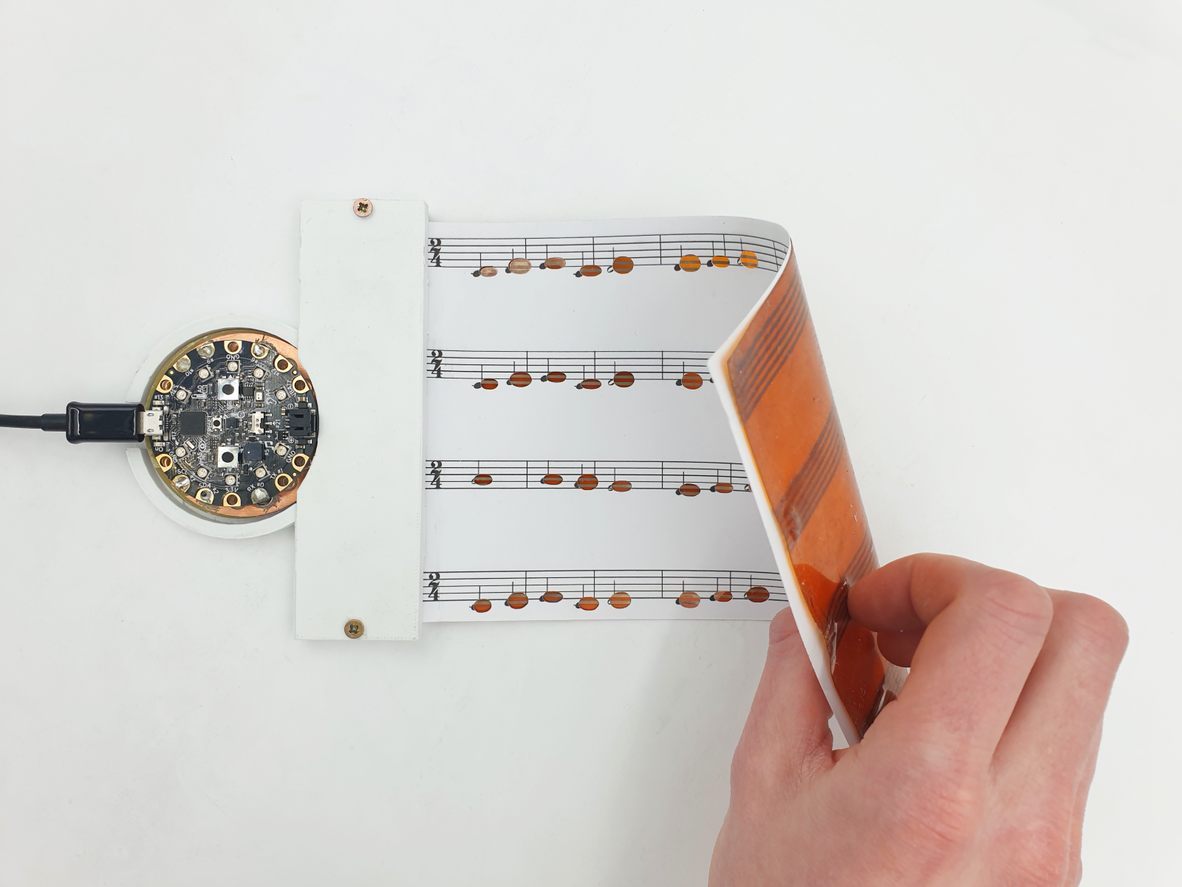
\includegraphics{images/IS_demo.png}
    \caption{Interactive Score Prototype}
    \label{fig:IS_demo}
\end{figure}

The user has to supply the electronic part (substrate and PCB), then he places a partition (a cardboard stencil) on top of the substrate (where
the conductive lines are located) \ref{fig:IS_demo}. He can play the music and change it to another one.

\subsection{System Design}

The Interactive score consists of two thin layers. The first layer is the traditional sheet
music, printed on cardstock paper, with holes punched for each note. Under this sheet
is a polyimide substrate with conductive lines printed on it \ref{fig:IS_schema}. 

\begin{figure}[h]
    \centering
    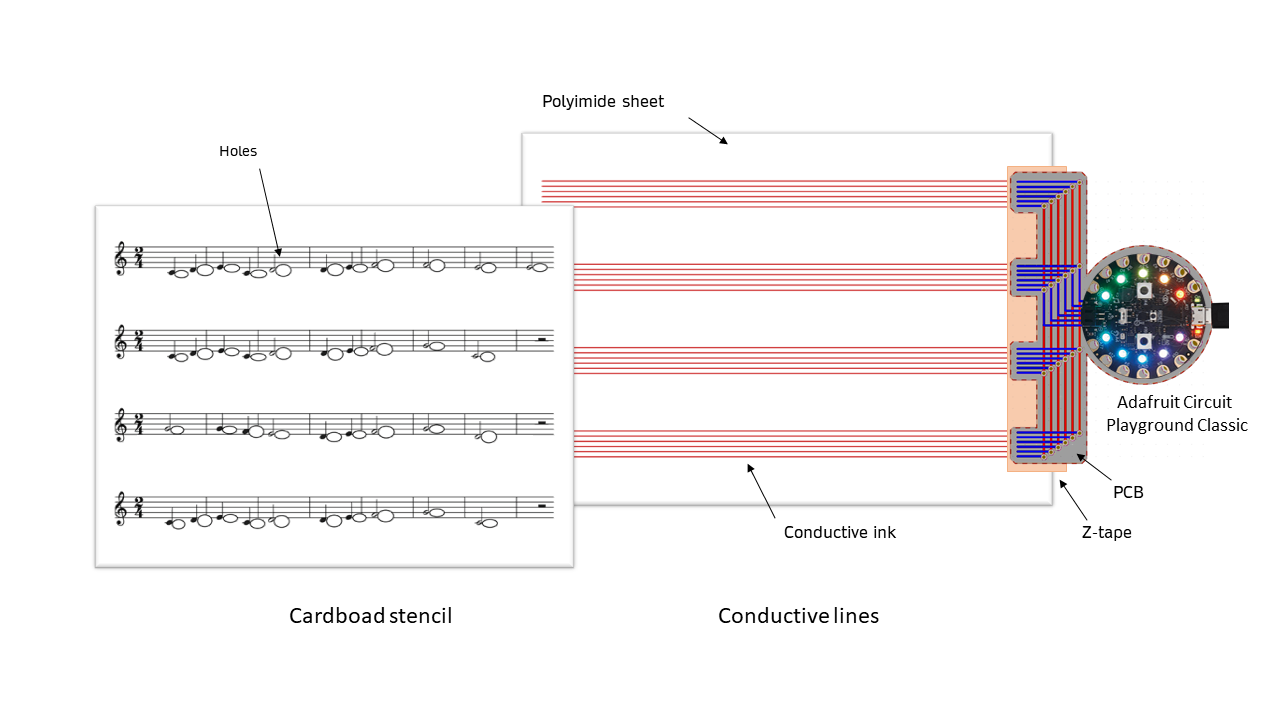
\includegraphics{images/IS_schema.png}
    \caption{Interactive Musical Score architecture.}
    \label{fig:IS_schema}
\end{figure}

The conductive lines are connected to an Adafruit Circuit Playground printed circuitnboard (PCB) using double-sided “z-tape”.

When the user touches a note on the top layer, contact is made between the finger and the conductive lines through the holes in the cardstock.
 The signal travels through the ink paths and the z-tape to the PCB, which detects a potential difference using capacitive touch and plays the relevant note. The detection of several simultaneous signals on multiple pins allows the playing of eleven different notes with only six lines \ref{fig:IS_schema}.

The whole system is kept in a 3D printed case, maintaining contact between the polyimide, the z tape, and the PCB. The case is designed to be easily opened and closed, allowing the user to change the music.



\subsection{Electronic Music Box}

The signal is recovered and used in capacitive touch with an Adafruit Circuit Playground Classic \ref{fig:circuit_playground_classic}. An Arduino program allows to generate a vast number of different notes. The code is retrievable on GitHub \cite{adrien2022capacitive_to_notes}.

\begin{marginfigure}
    \centering
    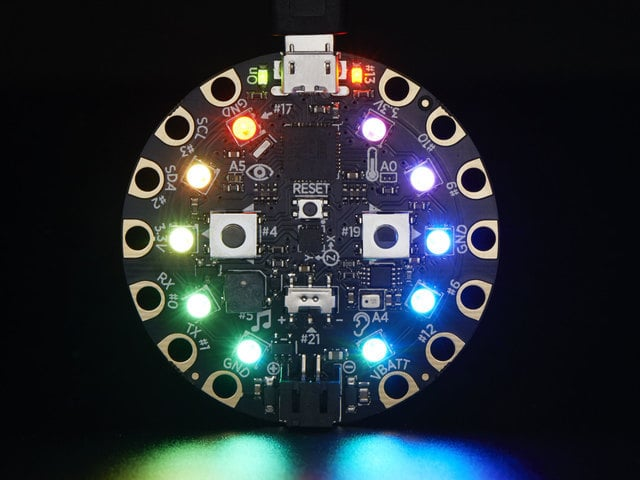
\includegraphics{images/circuit_playground_classic.jpg}
    \caption{Adafruit Circuit Playground Classic}
    \label{fig:circuit_playground_classic}
\end{marginfigure}

About the sound, the Adafruit Circuit Playground embarks a built in buzzer. The Mini Speaker that is implemented here is the SQMS5002S4036A. This device is a miniature magnetic speaker not adapted for playing detailed audio. It is more used for beeping and buzzing and for simple bleepy tunes. It is also possible to change the tone by changing the name of a variable in the code on the microcontroller.

The adafruit circuit playground has 10 mini NeoPixels of all colors, which can be animated with light when a note is played. The controller includes motion, temperature, light, and sound sensors, as well as a switch and a mini speaker. This device is therefore perfectly suited for use on the score and integrates many features in one.

\subsection{Paper Score Manufacturing}

For perfect dimensional compatibility between the different elements of the score, The music score printed on the stencil was entirely designed in PhotoShop. Notes, staves, lines, hyphenation, and cutouts were all placed on the same project. It allows the elements to fit together perfectly and export the cutout locations at the correct size relative to the partition's rest.

An inkjet printer draws all cardboard lines, hyphenation, notes, and numbers.

A score of "J'ai du bon tabac" (on the left) is positioned on the substrate. Then, the notes were isolated in another PNG file, selected on Cricut design, and cut directly into the cardboard with Cricut maker 3.

% TODO Justifier les choix techniques

\subsection{Conductive Sheet Manufacturing}

The conductive ink lines paths are 1mm thick, 5cm in length, with a resistance of 0.07 Ohms. The lines are printed using a simple inkjet printer equipped to print with silver nanoparticules conductive ink. The printed patterns are then sintered at 180°C for 73 minutes. This process allows the quick production of flexible circuits \cite{khan2019soft}.

\begin{figure}[h]
    \centering
    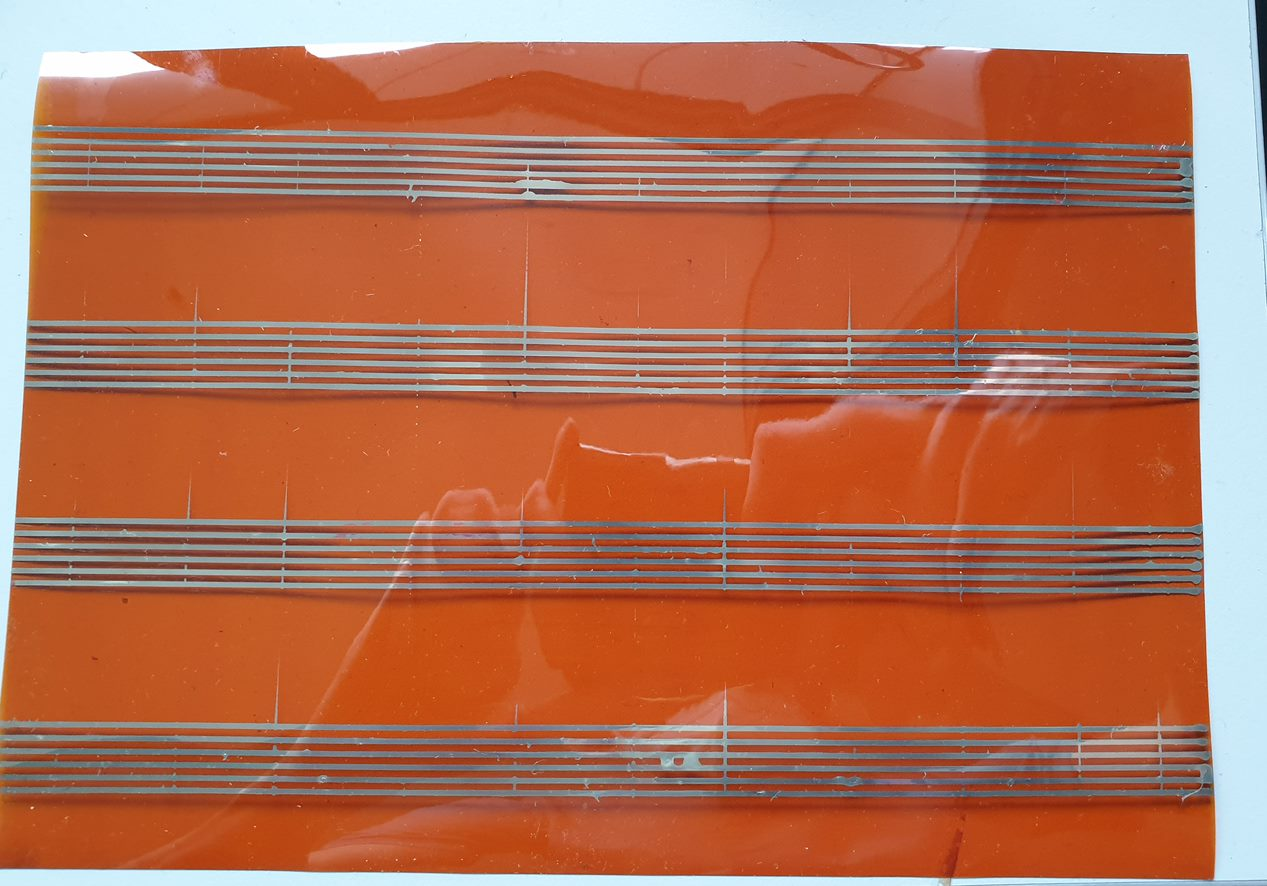
\includegraphics{images/IS_conductive_sheet.jpeg}
    \caption{Interactive Score Conductive Sheet}
    \label{fig:IS_conductive_sheet}
\end{figure}

This prototype comprises four staffs of 6 lines made of conductive ink on a Kapton polyimide sheet substrate. This polymer does not melt at high temperatures and has excellent mechanical strength, and is very dimensionally stable and creep resistant at temperatures above 260°C. The lines are 1mm thick, and at a distance of 15cm in length, it gave a resistance of 0.07 Ohms.

An Epson WF-2010 printer printed the lines on the substrate \cite{adrien2022capacitive_to_notes}.

The use of conductive ink allows the score to be flexible like a real musical score. The choice of ink rather than flexible brass strips is explained by the advantage of being able to print interactive scores on an industrial scale very quickly. The material needed is only simple printers as well as ink and cleaning products for the printers. This facilitates and accelerates the production possibilities.

\subsection{Integration and Usability}

\subsubsection{Ability to change the score}

Its ease of interchangeability characterizes the paper score. It is easy to produce. It
can easily be removed from the box and another one placed in its place to play a
different melody. All the electronic parts (substrate, PCB, microcontroller) are
independent of the paper score. The user can change it without changing the code or
the rest of the device. The sheet music has the exact dimensions of the substrate.
Therefore, it is simple to place the two precisely on top of each other to align the
holes with the ink lines.

\subsubsection{Ability to improvise} 

The user has the capacity to improvise by not playing the notes in the same order.
The project allows a great deal of modularity in its use. Just by touching specific
notes at certain times, users can experiment with different rhythms and melodies
and reconstruct a piece from a few notes.
With a simple score including an ascending scale, he can try his hand at composition.
As the microcontroller code is configured to play melodies in C major, it is not
possible to create dissonance.


\section{Applications and Evaluation}

\subsection{Set up}

Four users are selected at random. They interact with the prototype already prepared for use. They then answer several questions. The project is plugged in and set up as a base for further use. The users have tested the prototype. The project does not aim to teach a user how to play music. It seeks to link music theory directly with music practice without requiring knowledge.
It is difficult to test whether the project impacts the user's ability. Therefore, measuring the openness and visualization of music theory given by the project to the user is interesting. The questions concern understanding use, practicality, interest, innovation, attractiveness, and playfulness.

\subsection{Results}

The users did not encounter any particular problems during the test. The prototype worked well. The testers gave interesting feedback. As most of their comments have been taken into account since the last test, there were far fewer negative comments.

The users proposed many ideas to make the project evolve. They advised adding indications, potentially with LEDs, to indicate actions to be carried out. One idea was to create a binder with different stencils inside. They would have appreciated a correction of the electronics, which would warn them if they made a mistake. The people who tested the project were quite satisfied. They liked the fact that they could interact. The fact that the person playing presses the right notes and not that the sound automatically adapts to what they are doing was emphasized. It is because the sounds are corrected to play the right notes on some music toys, wherever the user presses (on the notes of a keyboard, for example). The users were also very interested in the fact that the project is portable. They would have liked to be able to take it with them to play music everywhere.

\section{Discussion}

\subsection{Attractivity}

The project is attractive for children as a tangible object. 
Its gamified aspect makes it close to a toy. This contributes to its attractiveness, especially to young children. Its musical property favors the creativity of the user, in addition to being portable, tactile, fun, and easy to use. 

\subsection{Musical Imagery learning}

An important aspect of musical practice is the ability of the musician to decipher a score. When this one practices with a visual support, his brain must take the exercise to connect the note which he links visually with the position of his fingers on the instrument. An intermediate used by the brain is the transcription of the note read, in its "mental", from which an interval and therefore a position is deduced. The ability to translate the visual note into a sound is therefore a reflex to be trained and very relevant in the practice of music. The basics of this ability must be acquired very quickly when learning the basics of music.

\subsection{Mobilising multiple intelligences}

This kind of device has a real interest in terms of learning. The user practices bodily intelligence with touch, the visual intelligence since he has a support in front of him, but also the musical-rhythmic intelligence.

\section{Conclusion}

In conclusion, the interactive score project has a bright future ahead of it, as it implements a very recent technology to popularize it. This process could be industrialized and even replicable for individuals, with some improvements and optimizations. In the future, our goal is to make the score more accessible. Features such as flexibility and simple "plug and play" aspect make it attractive even to children.

\subsection{Limitations}

The project has some limitations being a prototype. The device is limited in terms of the number of playable notes. The conductive sheet has six lines of conductive ink, which allows to play 13 different notes between C5 and F6. It is not possible to generate alterations while playing. This means that if the playground circuit is set in a specific key, it is not possible to play a note with an alteration that is not present in the score's framework. The key must also be changed manually at each score change (paper sheet).

The major problem of the prototype is in its transmission of electrical signals. 
The most important problem of the project is its sensitivity to electric field due to the use of capacitive touch. Near electric fields, the microcontroller can detect false contacts. The device must also be connected to a power outlet so that the potential difference calculated between the user's finger and the ground is remarkable. Otherwise, the playground circuit may not detect the touch of a line or start playing by itself because of the detection of surrounding electric fields. The device should therefore be used at a distance from electronic devices and metal surfaces.

The transmission of the signal from the conductive sheet to the PCB (inside the box) is done with z-tape. This conductive tape can be damaged and cause false contacts after many uses and transport. The current can then not be transmitted to the lines and some notes stop working. 

Another problem is also due to the conductive ink which can crumble, preventing the current from crossing certain lines. The ink traces are indeed quite fragile and easily damaged. The ink being only dried on the substrate, its adhesion is rather weak. As the user has to run his finger over the ink, he can also remove thin layers, thus causing some lines to break.

The prototype also presents a difficulty to overlay the sheet paper on top of the polyimide sheet to align the notes with the ink lines while keeping a flexible system. The case was specially designed for this purpose but is not very effective in practice. 

The device is also limited in terms of sound quality.
The speaker driver circuitry is an on/off transistor driver, so the device is only able to play square waves. It is also not the same loudness over all frequencies but is designed to be the loudest at around 4 KHz. The sound generated is shrill, very electronic and of poor quality. It can thus slow down the desire to practice and does not resemble the sound of an instrument.

\subsection{Future works}

To answer the problem of changing the key, one idea is to add the play of an alteration with three "buttons" usable thanks to the capacitive touch: flat, sharp and natural which can be played with the index finger of the left hand. This would allow the user to discover the notion of these three tools and their meaning. This would be an interesting tool that would add an improvisation capacity to the system.

A "musical tutorial" should be added so that the user can listen to the score's music before having to play it. This would allow the user to assimilate the musical rhythm (the time between playing each note) with the physical rhythm (the time between pressing notes).

The electronic PCB/microcontroller part should also be redesigned to no longer integrate an Adafruit Circuit Playground but a much smaller circuit entirely handmade. It would so be possible to
improve the speaker's quality and connect the device to Bluetooth or Wi-Fi to play music at a distance.
The next steps are also about looking for partnerships in children's education to research
experimentations on the impact of this interactive score on music assimilation. Several
parameters would be evaluated, such as the concentration level, playing time, and
knowledge retention. It is necessary to consider different strategies to transcript musical-rhythmic on this interactive score.